\begin{frame}
\begin{tabular}{cc}
\psset{xunit=0.75cm, yunit=0.75cm}
\begin{pspicture}(-3,-3)(3,3)
\renewcommand{\fcScreen}{[-1 -1 -1] 0}
%\pscustom*[linecolor=cyan]{%
%\fcPolyLineIIId{[-2 -2 0] [-2 2 0] [2 2 0] [2 -2 0] [-2 -2 0]}%
%}%
\pscustom*[linecolor=white]{%
\fcCurveIIId{0}{360}{[2 t cos mul 2 t sin mul 0]}%
}%
%\fcAxesIIId{2}{2}{2}
\fcBoxIIId[linecolor=gray!30, linewidth=0.3pt]{[2 2 2]}{[2 2 0]}{[2 -2 2]}{[-2 2 2]}%
\fcPlotIIIdXconst[linewidth=0.3pt, linecolor=\fcColorGraph]{iterationsX=15, iterationsY=15}{-2}{4 x x mul sub sqrt -1 mul}{2}{4 x x mul sub sqrt}{1 dict begin /rho x x mul y y mul  add sqrt def rho rho mul 2 rho  sub mul  0 max end}%
\fcPlotIIIdYconst[linewidth=0.3pt, linecolor=\fcColorGraph]{iterationsX=10, iterationsY=10}{4 y y mul sub sqrt -1 mul}{-2}{4 y y mul sub sqrt}{2}{1 dict begin /rho x x mul y y mul  add sqrt def rho rho mul 2 rho  sub mul  0 max end}%
\fcCurveIIId[linecolor=\fcColorGraph]{0}{360}{[2 t cos mul 2 t sin mul 0]}%
\end{pspicture}

%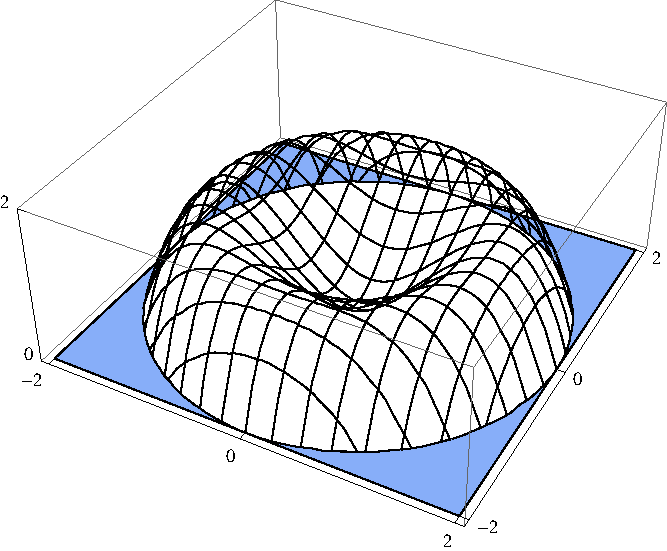
\includegraphics[height=4cm]{volumes/pictures/06-03-setup3d.pdf}%
&%
\psset{xunit=0.75cm, yunit=0.75cm}
\begin{pspicture}(-3,-3)(3,3)
\tiny%
\renewcommand{\fcScreen}{[-1 -1 -1] 0}%
\newcommand{\numIterations}{20\space}%
\pstVerb{%
100 dict begin
/numIterations \numIterations\space def
/goodAngleMin -50 def
/goodAngleMax 140 def
}%
\newcommand{\FunFla}{x x mul 2 mul x x x mul mul sub\space}%
\newcommand{\widthLine}{0.2pt}%
%\pscustom*[linecolor=cyan]{%
%\fcPolyLineIIId{[-2 -2 0] [-2 2 0] [2 2 0] [2 -2 0] [-2 -2 0]}%
%}%
%\pscustom*[linecolor=white]{%
%\fcCurveIIId{0}{360}{[2 t cos mul 2 t sin mul 0]}%
%}%
%\fcAxesIIId{2}{2}{2}%
%\fcStartIIIdScene%
%\fcSurfaceDirectDraw{}{}{}{}{}{}
%\fcFinishIIIdScene[true]%
\pstVerb{20 dict begin}%
\multido{\na=0+1}{\numIterations}{%
\pstVerb{%
/theCounter numIterations \na\space sub 1 sub def%
/theRad theCounter numIterations div 2 mul def
/theRadNext theCounter 1 add numIterations div 2 mul def
1 dict begin /x theRad def \FunFla end 
/theHeight exch def
1 dict begin /x theRadNext def \FunFla end 
/theHeightNext exch def
}%
%\pscustom*[linecolor=white]{%
%\fcCurveIIId{goodAngleMin 360 add}{goodAngleMax}{  [t cos theRad mul t sin theRad mul theHeight] }%
%\fcLineIIId{[goodAngleMax cos theRad mul goodAngleMax sin theRad mul theHeight]}{[goodAngleMax cos theRad mul goodAngleMax sin theRad mul theHeightNext]}%
%\fcCurveIIId{goodAngleMax}{goodAngleMin 360 add}{  [t cos theRad mul t sin theRad mul theHeightNext] }%
%\fcLineIIId{[goodAngleMin cos theRad mul goodAngleMin sin theRad mul theHeightNext]}{[goodAngleMin cos theRad mul goodAngleMin sin theRad mul theHeight]}%
%}%
\fcCurveIIId[linecolor=red, linewidth=\widthLine]{goodAngleMin 360 add}{goodAngleMax}{  [t cos theRad mul t sin theRad mul theHeight] }%
%\fcLineIIId[linecolor=\fcColorGraph]{[goodAngleMax cos theRad mul goodAngleMax sin theRad mul theHeight]}{[goodAngleMax cos theRad mul goodAngleMax sin theRad mul theHeightNext]}%
\fcCurveIIId[linecolor=red, linewidth=\widthLine]{goodAngleMin 360 add }{goodAngleMax}{  [t cos theRad mul t sin theRad mul theHeightNext] }%
%\fcLineIIId[linecolor=\fcColorGraph]{[goodAngleMin cos theRad mul goodAngleMin sin theRad mul theHeightNext]}{[goodAngleMin cos theRad mul goodAngleMin sin theRad mul theHeight]}%
}%
\multido{\nb=0+1}{\numIterations}{%
\pstVerb{%
/theCounter \nb\space def%
/theRad theCounter numIterations div 2 mul def
/theRadNext theCounter 1 add numIterations div 2 mul def
1 dict begin /x theRad def \FunFla end 
/theHeight exch def
1 dict begin /x theRadNext def \FunFla end 
/theHeightNext exch def
}%
%\pscustom*[linecolor=white]{%
%\fcCurveIIId{goodAngleMin}{goodAngleMax}{  [t cos theRad mul t sin theRad mul theHeight] }%
%\fcLineIIId{[goodAngleMax cos theRad mul goodAngleMax sin theRad mul theHeight]}{[goodAngleMax cos theRad mul goodAngleMax sin theRad mul theHeightNext]}%
%\fcCurveIIId{goodAngleMax}{goodAngleMin}{[t cos theRad mul t sin theRad mul theHeightNext]}%
%\fcLineIIId{    [goodAngleMin cos theRad mul goodAngleMin sin theRad mul theHeightNext]}{[goodAngleMin cos theRad mul goodAngleMin sin theRad mul theHeight]}%
%}%
\fcCurveIIId[linecolor=red, linewidth=\widthLine]{goodAngleMin }{goodAngleMax}{  [t cos theRad mul t sin theRad mul theHeight] }%
%\fcLineIIId[linecolor=\fcColorGraph, linewidth=0.4pt]{[goodAngleMax cos theRad mul goodAngleMax sin theRad mul theHeight]}{[goodAngleMax cos theRad mul goodAngleMax sin theRad mul theHeightNext]}%
\fcCurveIIId[linecolor=red, linewidth=\widthLine]{goodAngleMax }{goodAngleMin}{  [t cos theRad mul t sin theRad mul theHeightNext] }%
%\fcLineIIId[linecolor=\fcColorGraph, linewidth=0.2pt]{[goodAngleMin cos theRad mul goodAngleMin sin theRad mul theHeightNext]}{[goodAngleMin cos theRad mul goodAngleMin sin theRad mul theHeight]}%
}%
\pstVerb{end}%
\fcBoxIIId[linewidth=0.2pt, linecolor=gray!30]{[2 2 2]}{[2 2 0]}{[2 -2 2]}{[-2 2 2]}%
\fcCurveIIId[linecolor=\fcColorGraph]{0}{360}{[2 t cos mul 2 t sin mul 0]}%
\pstVerb{end}%
\end{pspicture}
%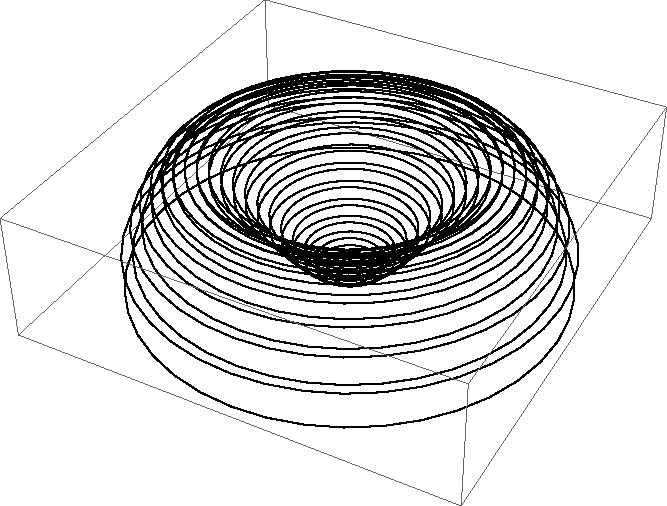
\includegraphics[height=4cm]{volumes/pictures/06-03-setupcylinders.pdf}%
\end{tabular}
\begin{itemize}
\item<1->  Consider the solid obtained by rotating around the $y$-axis the region bounded above by $y = 2x^2 - x^3$ and below by the $x$-axis.
\item<2->  Approximate this solid by nested cylindrical shells.
\item<3->  Cylindrical shells are solids obtained by taking a cylinder and removing from its center another cylinder of equal height but smaller radius.
\end{itemize}
\end{frame}